\clearpage
\section*{Systemtheorie der Sinnesorgane}
\subsection{Übung}
\subsubsection{}
For the underlying problem, we constructed a sinusoidal wave with an amplitude of $u_{max} = \SI{1}{\volt}$ around the steady component of $u_{DC} = \SI{0.5}{\volt}$. Thereby, the frequency of the oscillation was set to $f = \SI{1}{Hz}$ in the time interval of $t \in [0,\ 2]\ \si{s}$. For further analyses, a sampling frequency of $f_s = \SI{20}{Hz}$ was chosen. The sampling points are depicted as squares (Fig. \ref{fig:signal}).
\begin{figure}[h] 
  \centering
  \includegraphics[scale=1]{ue1/signal.eps} % oder statt scale auch [width=0.5\textwidth] für eine feste Größe
  \caption{Sinusoidal base signal for further analysis. The wave was constructed after $u(t) = u_{max} \mathrm{sin}(\omega t) +u_{DC}$ with $\omega = 2\pi f$.}
  \label{fig:signal}
\end{figure}
\subsubsection{}
In this exercise, the signal should be decomposed into its underlying frequencies by a Discrete Fourier Transformation (DFT), in this case Fast Fourier Transformation (FFT), to a single-sided amplitude spectrum. We are allowed to reduce the complete spectrum, because the transformed signal $u(t)$ is real and hence the relation $U(f)\ =\ U(-f)^*$ is valid. In this context, $a^*$ expresses the complex conjugation of $a$.

As the amplitude spectrum depicts the amplitudes of the composing waves, we can expect the amplitude of 1 at \SI{1}{Hz} created by our generating parameters $u_{max}$ and $f$. Further, the steady component $u_{DC}$ can be expressed as a wave with no frequency, but 0.5 amplitude. The composition of these two then forms $u(t)$.

\begin{figure}[h] 
  \centering
  \includegraphics[scale=1]{ue1/amp_fft.eps} % oder statt scale auch [width=0.5\textwidth] für eine feste Größe
  \caption{Single-sided FFT amplitude spectrum of the input signal $u(t)$.}
  \label{fig:amp_fft}
\end{figure}

\clearpage
\subsubsection{}
Subsequently, the voltage level of input signal $u(t)$ was computed using equation \ref{eq:sp_pegel} and is shown in figure \ref{fig:Lu_sig}. \SI{1}{V} was selected as reference voltage level $U_0$. A Fourier transformation to the voltage spectrum (shown in Fig. \ref{fig:Lu_fft}) shows many more different frequencies overlapping to the signal.
\begin{alignat}{2}
    &L_U\ &&=\ 20\ \mathrm{log}_{10}\left(\frac{U}{U_0}\right)\ \si{dBV} \label{eq:sp_pegel}\\
    RMS&(L_U)\ &&=\ L_{U,eff}\ =\ \sqrt{\frac{1}{T}\int_{t_0}^{t_0+T}L_U^2dt} \label{eq:RMS_cont} \\
    &&&\underset{equidist.\ grid}{\overset{discretized}{=}}\ \sqrt{\frac{1}{N}\sum_{n=1}^{N}|L_{Ui}|^2} \label{eq:RMS}
\end{alignat}
\begin{figure}[h] 
  \centering
  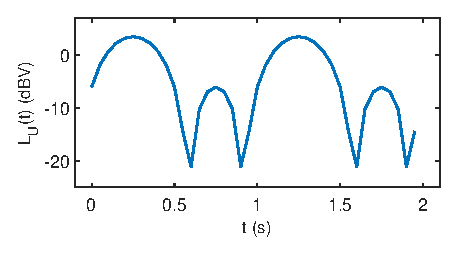
\includegraphics[scale=1]{ue1/L_U_sig.eps} % oder statt scale auch [width=0.5\textwidth] für eine feste Größe
  \caption{Voltage level computation after eq.\ref{eq:sp_pegel} from $u(t)$ to the reference voltage $U_0=\SI{1}{V}$}
  \label{fig:Lu_sig}
\end{figure}

\begin{figure}[h] 
  \centering
  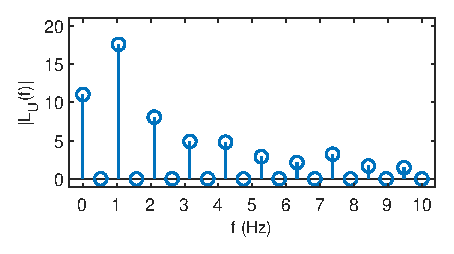
\includegraphics[scale=1]{ue1/L_U_fft.eps} % oder statt scale auch [width=0.5\textwidth] für eine feste Größe
  \caption{Single-sided FFT-spectrum of $L_U$}
  \label{fig:Lu_fft}
\end{figure}
Additionally, the Root-Mean-Square (RMS) was calculated according to equation \ref{eq:RMS}. To achieve this, we discretized the continuous integral in eq. \ref{eq:RMS_cont} with $T\ =\ n \cdot \Delta t$ under the assumption of constant time steps. Plugging the values of $L_U$ into the equation above gives a RMS of 18.69.